% -*- coding: utf-8; -*-

\chapter{Introdução}
\label{ch:intro}
	Visualização volumétrica é a vertente da computação gráfica caracterizada por visualizar campos escalares tridimensionais, isto é, representar visualmente um volume de dados que relaciona um valor escalar a um ponto no espaço. Esses dados podem vir de inúmeras fontes, desde exames médicos de ressonância magnética (RM) e tomografia computadorizada (TC) a simulações físicas, como simulação numérica de reservatórios de petróleo e análise de fraturas em materiais. Um campo escalar também pode ser interpretado como a variação de uma determinada informação num espaço delimitado. Por exemplo, um exame de tomografia computadorizada informa como a densidade da estrutura fisiológica varia naquela região em que foi escaneada, como visto na Figura~\ref{fig:head_ct_slice_intro}, onde a cor preta indica a menor densidade e a cor branca a maior.
    
    Um componente essencial da visualização volumétrica é a função de transferência (FT): um mapeamento feito entre voxels do volume renderizado e um ou mais atributos que compõem suas propriedades ópticas, como por exemplo, cor e opacidade. Ou seja, através da função de transferência é possível definir como cada elemento do volume de dados será visto na imagem final. Um objetivo prático do uso de FTs seria, dado uma TC da cabeça de um indivíduo, visualizar apenas seu crânio. Essa prática auxilia os médicos no exame e diagnóstico de pacientes, o que mostra o quanto pode ser importante utilizar funções de transferência adequadas. As imagens na Figura~\ref{fig:head_skull_intro} mostram visualizações volumétricas da tomografia apresentada na Figura~\ref{fig:head_ct_slice_intro}, utilizando diferentes funções de transferência.
    
\begin{figure}[h]
	\centering
	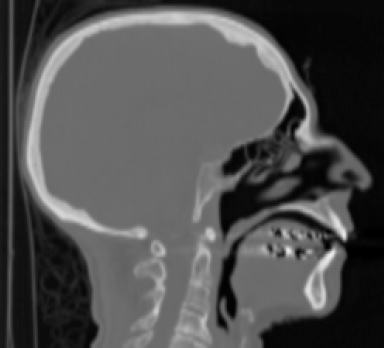
\includegraphics[width=0.3\textwidth]{images/head_ct_slice_intro}
    \caption{Uma imagem de tomografia computadorizada da cabeça de um indivíduo~\cite{gordonms}.}
    \label{fig:head_ct_slice_intro}
\end{figure}
\begin{figure}[h]
	\centering
    \subfigure[]{
    	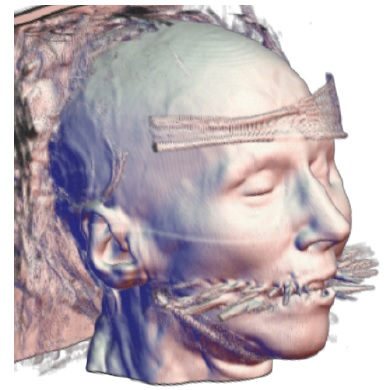
\includegraphics[width=0.3\textwidth]{images/head_ct_intro}
    }
    \subfigure[]{
    	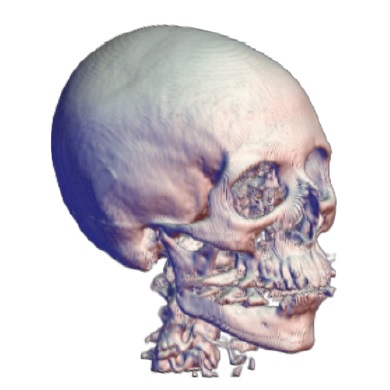
\includegraphics[width=0.3\textwidth]{images/head_skull_intro}
    }
    \caption{Visualização volumétrica de uma TC~\cite{gordonms}.}
    \label{fig:head_skull_intro}
\end{figure}
    
    No entanto, obter FTs que isolem corretamente estruturas internas do volume, ou que simplesmente resultem em uma visualização adequada de toda a estrutura de interesse, não é uma tarefa fácil para um usuário comum. Definir manualmente uma função de transferência é um trabalho repetitivo de tentativa e erro, que exige paciência e um conhecimento sobre os dados sendo visualizados. Por esse motivo, a busca por métodos automáticos para a definição de FTs é tão importante e vem sendo desenvolvida há mais de 20 anos.
    
    Em 1998, \textit{Kindlmann e Durkin}~\cite{gordon} aprimoraram a obtenção de funções de transferência para as fronteiras entre materiais distintos. Alguns trabalhos que vieram a seguir buscaram o mesmo objetivo: automatizar a criação de FTs que destacassem as fronteiras entre diferentes materiais do volume, permitindo ao usuário um controle fino sobre a função obtida. Mas a maioria das pesquisas que se sucedeu resultou em um aprimoramento da interface com o usuário, explorando mais interatividade. Através de histogramas 2D, regiões de possíveis fronteiras são reveladas, cabendo então ao usuário selecioná-las, atribuindo cor e opacidade~\cite{haidacher, sereda1, wang, zou}.
    
    Esse tipo de abordagem dá ao usuário controle total sobre a função de transferência que será gerada, ao mesmo tempo que as interfaces sofisticadas minimizam a necessidade de se conhecer os dados sendo visualizados. Contudo, esses trabalhos retomam o processo repetitivo de tentativa e erro. Além disso, como a relação entre as regiões dos histogramas e os materiais do volume não são intuitivas, a interface apresenta um novo desafio cognitivo ao usuário.
    
    Durante esses anos, a grande maioria das pesquisas tem analisado seus resultados em volumes provenientes de exames médicos, ou de métodos de aquisição semelhantes. Como consequência, os trabalhos desenvolvidos exploram apenas malhas regulares, deixando de lado dados representados por malhas não regulares e não estruturadas. Os dados de simulação numérica de reservatórios de petróleo, por exemplo, são representados por malhas não regulares e, portanto, representam uma área na qual as funções de transferência ainda não foram exploradas.
    
    Segundo \textit{Rosa et al.}~\cite{rosa}, a simulação numérica é um dos métodos mais sofisticados para se estimar características e prever o comportamento de reservatórios de petróleo. A simulação permite, por exemplo, determinar as melhores condições para a produção de petróleo, bem como estimar o volume de óleo e gás que poderá ser extraído durante a exploração do reservatório. Assim como no caso dos volumes médicos, a simulação numérica de um reservatório resulta em campos escalares 3D, o que permite a aplicação de funções de transferência para destacar a interface entre diferentes regiões do reservatório. Por exemplo, a área de contato entre a água e o óleo (denominada frente de avanço) é uma informação importante sobre o fluxo do reservatório.
    
    As frentes de avanço delimitam regiões importantes na fase de recuperação secundária de um reservatório, mas não podem visualizadas sem uma função de transferência apropriada. A Figura~\ref{fig:reserv_livro} mostra a frente de avanço da área invadida pela água em quatro momentos diferentes. O modelo em questão é um reservatório cúbico com um poço injetor no canto inferior esquerdo e um poço produtor no canto diagonal oposto. A simulação de um reservatório com as mesmas características pode ser observada na Figura~\ref{fig:reserv}, onde \ref{fig:reserv_intro} mostra a simulação da saturação de óleo do reservatório em um dado tempo, enquanto \ref{fig:reserv_tf_intro} mostra a visualização da frente de avanço identificada nesse mesmo tempo, através de uma FT.
    
\begin{figure}[h]
   	\centering
   	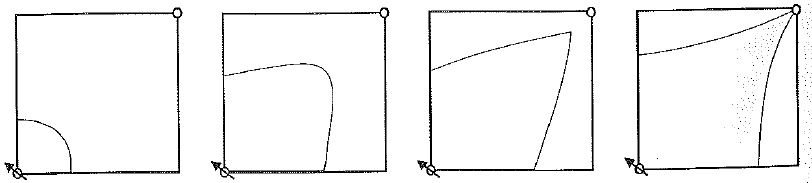
\includegraphics[width=1\textwidth]{images/reserv_livro}
   	\caption{Evolução da área invadida em uma malha de 5 pontos~\cite{rosa}.}
   	\label{fig:reserv_livro}
\end{figure}
    
\begin{figure}[h]
	\centering
    \subfigure[Simulação da saturação de óleo em um reservatório.]{
    	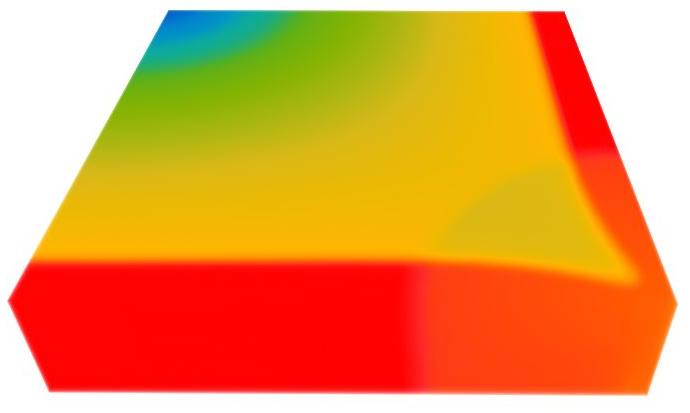
\includegraphics[width=0.35\textwidth]{images/reserv_intro}
        \label{fig:reserv_intro}
    }
    \subfigure[Realce da fronteira mais evidente da imagem ao lado.]{
    	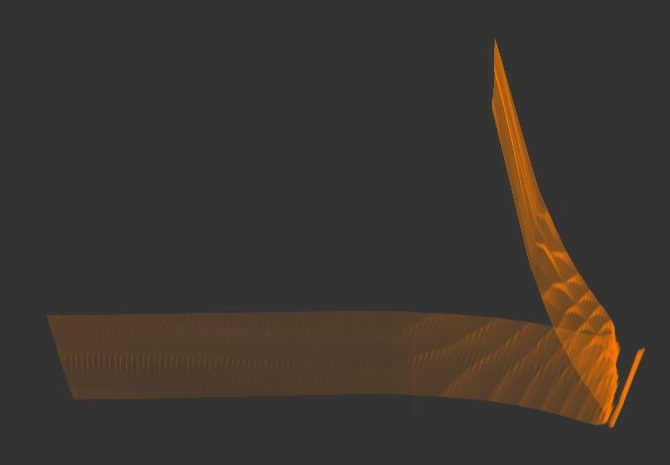
\includegraphics[width=0.35\textwidth]{images/reserv_tf_intro}
        \label{fig:reserv_tf_intro}
    }
    \caption{Visualização volumétrica de reservatório de petróleo.}
   	\label{fig:reserv}
\end{figure}
    
    Com base na abordagem feita por \textit{Kindlmann e Durkin}~\cite{gordon}, este trabalho desenvolve um novo método para geração automática de funções de transferência, com o objetivo de realçar fronteiras de um volume de dados, tendo também como diferencial a aplicabilidade em malhas não regulares. A técnica desenvolvida utiliza a terceira derivada média para encontrar as intensidades do volume de dados que melhor representam o centro das fronteiras existentes. A partir dos valores encontrados, uma função de transferência baseada em gaussianas é automaticamente gerada, podendo ser modificada pelo usuário através da interface desenvolvida.
    
    As principais contribuições desta dissertação são:
\begin{itemize}
   	\item Releitura detalhada e análise do método proposto por \textit{Kindlmann e Durkin}~\cite{gordon}.
   	\item Definição de uma regra para encontrar automaticamente valores de $ g_{thresh} $ para o trabalho de \textit{Kindlmann e Durkin}~\cite{gordon}.
   	\item Proposta de um novo método para gerar FTs automaticamente.
\end{itemize}

    No Capítulo \ref{ch:related} alguns trabalhos relacionados a este são comentados, realçando suas contribuições e questões em aberto que deram espaço a outros trabalhos. No Capítulo \ref{ch:gordon}, o método criado por \textit{Kindlmann e Durkin}~\cite{gordon} é explicado e avaliado segundo os objetivos e motivações deste trabalho. A abordagem proposta por essa dissertação é apresentada no Capítulo \ref{ch:my} e seus resultados e comparações avaliados no Capítulo \ref{ch:result}, através de volumes sintéticos, volumes médicos e volumes de reservatório. Por fim, conclusões e trabalhos futuros são discutidos no Capítulo \ref{ch:conclusion}.